%!TEX root = ../pres - final.tex

\section{Speaker Diarization}

\subsection{Formulación matemática}
\begin{frame}{Formulación matemática (I)}
Denótese por $\mathcal{A}$ la evidencia acústica a partir de la cuál el modelo deberá encontrar la segmentación correcta para un fragmento de señal.
\\~\\
Se puede pensar en $\mathcal{A}$ como la secuencia de símbolos correspondiente a un segmento de señal, y que está conformada por elementos de un alfabeto mucho más grande $\mathbb{A}$. 
\begin{equation}
\mathcal{A} = a_1, a_2, ..., a_K \quad a_i \in \mathbb{A}
\label{eqn:2a-1}
\end{equation}
en donde los elementos $a_i$ hacen referencia a un intervalo de tiempo $i$ en la secuencia de audio original.
%, y los valores que tomen pueden repetirse de acuerdo a la grabación.
\vfill
De la misma manera,
\begin{equation}
\mathcal{S} = s_1, s_2, ..., s_N \quad s_i \in \mathbb{S}
\label{eqn:2a-2}
\end{equation}
donde $\mathcal{S}$ es la secuencia que corresponde a la segmentación correcta para un intervalo del audio original. 
\\~\\
$\mathbb{S}$ es el conjunto de todos los interlocutores que participan en la grabación de audio y $s_i$ de igual manera representa al interlocutor que habla en el tiempo $i$.
\end{frame}

\begin{frame}{Formulación matemática (II)}
Si $P(\mathcal{S} \,|\, \mathcal{A})$ es la probabilidad de que una secuencia de interlocutores $\mathcal{S}$ esté hablando dada la evidencia acústica en $\mathcal{A}$, entonces para escoger cuáles son los personas que hablan en ese intervalo se calcula:
\begin{equation}
\hat{\mathcal{S}} = \underset{\mathcal{S}}{arg~max}~ P(\mathcal{S} \,|\, \mathcal{A})
\label{eqn:2a-3}
\end{equation}
%Seleccionaría la sucesión de interlocutores más probable para una secuencia de datos dada.
%\\~\\
\vfill
Que por el Teorema de Bayes, es equivalente a maximizar: 
\begin{equation}
\hat{\mathcal{S}} = \underset{\mathcal{S}}{arg~max}~ P(\mathcal{S}) \cdot P(\mathcal{A} \,|\, \mathcal{S})
\label{eqn:2a-6}
\end{equation}
pues la variable $\mathcal{A}$ es constante respecto a $\mathcal{S}$. %-pues es la única evidencia acústica observada-

\end{frame}

\subsection{Componentes del sistema (I)}
\begin{frame}{Componentes del sistema}
  En general, todos los sistemas que involucran procesamiento de
  voz, tienen varias etapas esenciales, como se menciona en Jelinek (cita)

  \begin{enumerate}
    \itemsep1em
    \item \structure{Procesamiento acústico:}
    Se refiere a la forma en la que se procesará la información y se digitalizará.% Usualmente se contará con un micrófono o un arreglo de micrófonos que captarán las voces y las transformarán en impulsos eléctricos. 
    %\\~\\
    Además se debe realizar algún proceso para obtener una representación paramétrica de la señal. A este procedimiento se le conoce como construcción del \textit{diccionario de palabras}.

    \item \structure{Modelado acústico:}
    Se considera que ya se ha construido el diccionario de palabras o la evidencia acústica $\mathbb{A}$, y se necesita proponer una forma de calcular las probabilidades $P(\mathcal{A} \,|\, \mathcal{S})$. 
    % \\~\\
    El modelo acústico más comúnmente utilizado en tareas de procesamiento de voz, es el HMM, aunque hay trabajos que utilizan otras técnicas: ANN \cite{Jothilakshmi2009} \cite{Gutzwiller2010}  o métodos de DTW \cite{Huijbregts2011} 
  \end{enumerate}

\end{frame}

\begin{frame}{Componentes del sistema (II)}
  \begin{enumerate}
    \item \structure{Modelado de interlocutores:}
    \item \structure{Búsqueda de hipótesis:}
  \end{enumerate}

\end{frame}

\subsection{Procesamiento acústico}

\begin{frame}{Elminación de ruido / Detección de silencios}
  \begin{center}
    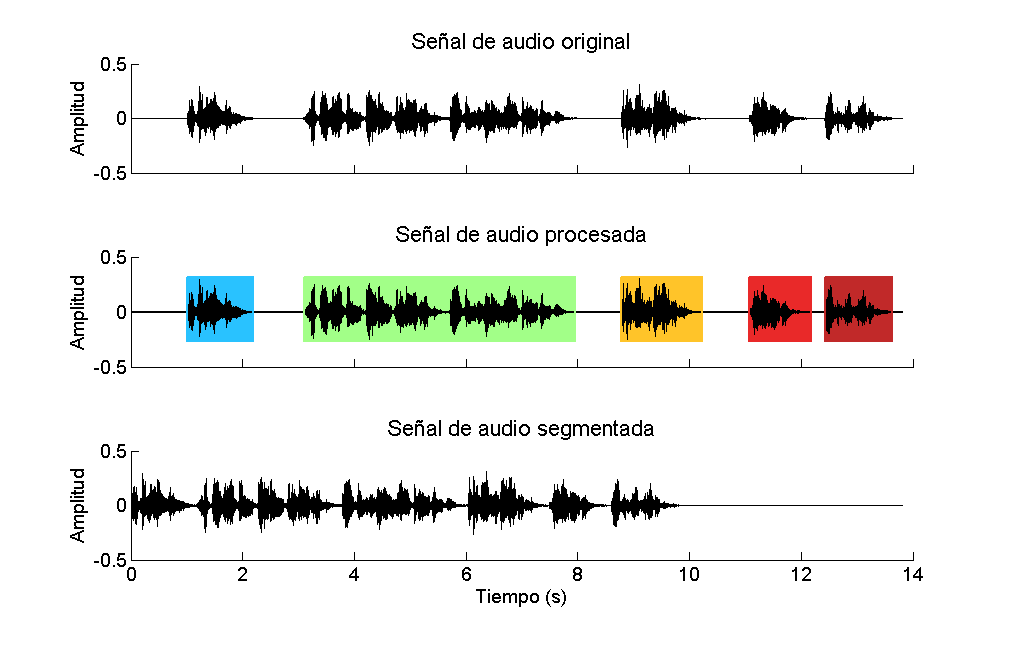
\includegraphics[width=1\textwidth]{gfx/f-silence}
  \end{center}
\end{frame}

%\subsubsection{Obtención de vector de características}

\begin{frame}{Mel Frequency Cepstrum Coefficient}
  \begin{itemize}
    \item \small{FFT (ventana) -> Banco de filtros triangular (Mel Scale) -> Log -> DCT -> MFCC}
  \end{itemize} 
  \begin{center}
    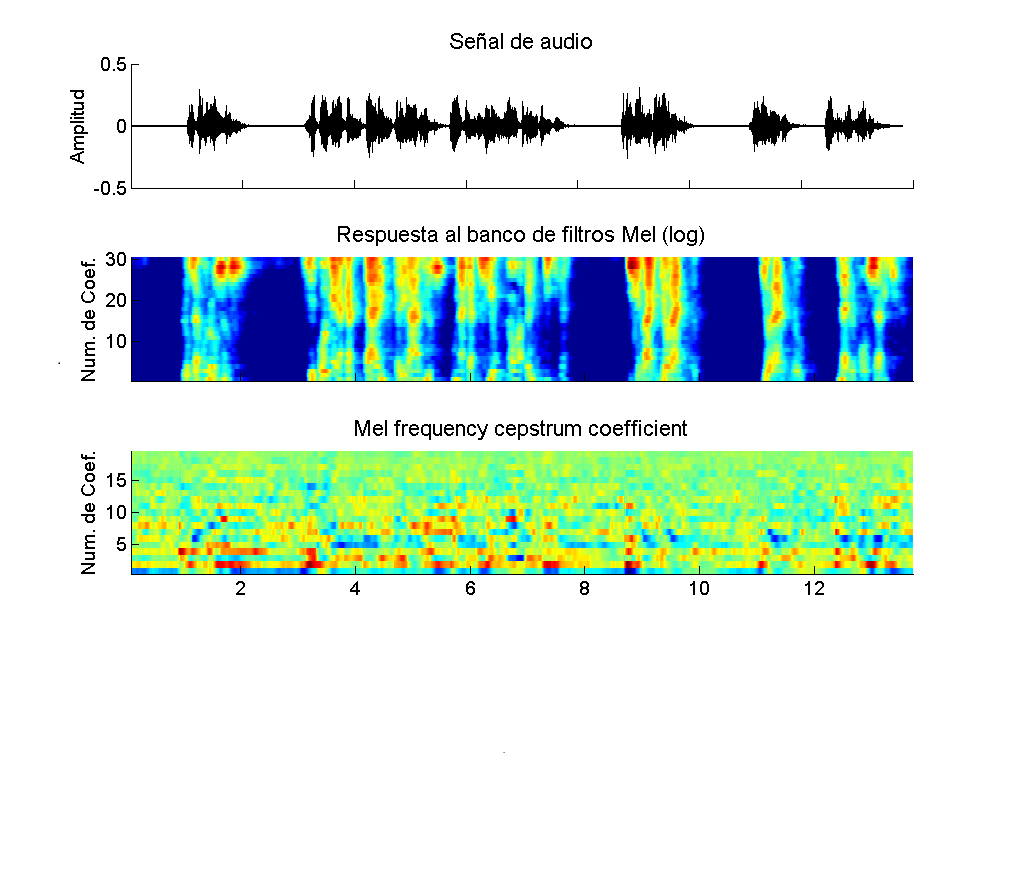
\includegraphics[width=1\textwidth]{gfx/f-mfcc}
  \end{center}
\end{frame}